\documentclass[a4paper,12pt]{article}

\usepackage[french]{babel}   % Active la langue française
\usepackage{graphicx}    	% Pour insérer des images
\usepackage{lipsum}      	% Pour du texte factice
\usepackage{fancyhdr}    	% Pour personnaliser les en-têtes et pieds de page
\usepackage{listings}    	% Pour afficher le code
\usepackage{xcolor}      	% Pour personnaliser les couleurs
\usepackage{minted}      	% Pour une coloration syntaxique avancée
\usepackage{amsmath}     	% Pour les équations
\usepackage{hyperref}    	% Pour les liens cliquables
\usepackage{tcolorbox}
\usepackage{lmodern}


\hypersetup{
	colorlinks=true,   	% Active les liens en couleur
	linkcolor=blue,    	% Couleur des liens internes
	urlcolor=blue,     	% Couleur des liens externes
	citecolor=blue     	% Couleur des liens de citation
}



\pagestyle{fancy}  % Active le style personnalisé
\fancyhf{}  % Efface les en-têtes et pieds de page par défaut


\fancyfoot[R]{
\includegraphics[width=1.3cm]{logo.png}}


% Ajouter la numérotation des pages à droite du pied de page
\fancyfoot[C]{\thepage}

\renewcommand{\sectionmark}[1]{\markboth{#1}{}}

% Afficher la section courante à gauche du pied de page
\fancyfoot[L]{\nouppercase{\leftmark}}

\begin{document}

% ---- Page de titre ----
\begin{titlepage}
	\centering
	
\includegraphics[width=4cm]{logo.png} \\[1cm]  % Ajuste la taille du logo

	{\LARGE \textbf{Etude de la dynamique des foules}} \\[0.5cm]
    
	{\large Par le biais de la physique moderne} \\[1.5cm]

	\textbf{Auteurs :} \\[0.3cm]
	NADAUD Antonin \\
	JANINI  Raphaël \\
	LUBIN Thomas \\
	NUCE LAMOTHE Augustin \\[1cm]

	\textbf{Encadrant :} \\[0.3cm]
	DESPLAT Lucie \\[1.5cm]

	\textbf{\today}  % Affiche la date du jour
	\\[2cm]

	\vfill % Remplit l'espace verticalement pour centrer

	{\large CY Tech – préing-2 groupe 2} \\

\end{titlepage}

% --- page blanche ---
\newpage
\thispagestyle{empty}  % Pas de numérotation, ni d'en-tête/pied de page
\mbox{}  % Crée une page vide (avec un espace vide)

% ---- Sommaire ----
\newpage


\renewcommand{\contentsname}{Sommaire}  % Change "Contents" en "Sommaire"
\thispagestyle{empty}
\tableofcontents  % Génère le sommaire automatiquement avec des liens cliquables

% ---- introduction --- 
\newpage

\setcounter{page}{1} % -- met la page à 1 --

\section{Objectif}

Cette étude s’inscrit dans le cadre d’un travail de foulométrie, visant à modéliser et analyser les dynamiques d’évacuation d’un groupe d’individus dans des environnements clos. À travers différentes configurations, nous cherchons à comprendre l’impact de la configuration des lieux sur le temps d’évacuation global. Deux scénarios ont été étudiés dans cette analyse.

\subsection{Évacuation depuis une salle unique}

Dans ce second scénario, on a deux salles identiques, mais leurs nombres de sortie est différent. En effet la salle 1 dispose d’une seule porte, tandis que la salle 2 en a deux. Les deux espaces accueillent 31 personnes (composés d'un professeur et d'étudiants).
L’objectif est ici de quantifier l’impact de la présence d’une issue supplémentaire sur l’efficacité de l’évacuation, en comparant les temps d’évacuation des deux configurations.

\subsection{Comparaison entre une et deux issues de secours}

Dans ce second scénario, on a deux salles identiques, à l’exception du nombre de sorties : la salle 1 dispose d’une seule porte, tandis que la salle 2 en possède deux. Les deux espaces accueillent un total de 31 individus (composés d'un professeur et d'étudiants).
L’objectif est ici de quantifier l’impact de la présence d’une issue supplémentaire sur l’efficacité de l’évacuation, en comparant les temps d’évacuation des deux configurations.
\
\section{Théorie sous-jacente}

Nous nous somme appuyé sur les travaux du modèle de force sociale, de Helbing et Molnár
\footnote{Lien vers l'étude \url{https://doi.org/10.1103/PhysRevE.51.4282}}
, visant à simuler le comportement de piétons dans des foules. Il y a deux forces principales dans ce modèle : la force motrice et la force d'interaction.

\paragraph{Force motrice.}
Chaque individu $i$ cherche à atteindre une vitesse souhaitée $\vec{v}_i^0$ dans une direction donnée. Ce comportement est modélisé par une force motrice, qui pousse l'individu à ajuster sa vitesse actuelle $\vec{v}_i$ à sa vitesse désirée, selon :

\begin{equation}
\label{eq:force_motrice}
\vec{f}_i^{\text{m}} = m_i \frac{\vec{v}_i^0 - \vec{v}_i}{\tau_i}
\end{equation}

où $m_i$ est la masse de l'individu et $\tau_i$ est le temps de relaxation modélisant la rapidité avec laquelle l'individu peut atteindre sa vitesse cible.

\paragraph{Force interaction.}
Les piétons interagissent entre eux via des forces dites sociales, traduisant leur tendance à maintenir une distance avec d'autres personnes, aussi les piètons intéragissent avec l'environnement avec des forces dites d'intércation. Ces interactions sont traduites par la même modélisation:

\begin{equation}
\label{eq:force_sociale}
\vec{f}_{ij}^{\text{s}} = A_i \exp\left(\frac{r_{ij} - d_{ij}}{B_i}\right) \vec{n}_{ij}
\end{equation}

où :
\begin{itemize}
  \item  $B_i$ est une constantes ( la zone de confort de la personne i),
  \item $r_{ij}$ est la somme des rayons des individus respectifs $i$ et $j$,
  \item $d_{ij}$ est la distance entre les centres des deux individus (ou individu masse),
  \item $\vec{n}_{ij}$ est le vecteur unitaire (de $j$ vers $i$).
\end{itemize}

Ces forces permettent de modéliser des comportements réalistes d’évitement.


\section{Méthode}

\subsection{Determiner l'équation}

\indent Afin d’établir l’équation, nous avons tout d’abord supposé que le référentiel d’étude est galiléen, pour ensuite appliquer la seconde loi de newton $\sum \vec{F}_{\text{particule}} = m_{\text{particule}} \vec{a}$.
\\(on ne considère pas le poid ni la réaction du support car selon $\vec{e_z}$)
\\ On a:
\[
\vec{f}_{\text{direction}} + \vec{f}_{\text{social}} = m_{\text{particule}} \frac{d\vec{v}}{dt}.
\]
\\ Au final après quelques simplification on a:

\begin{equation}
\label{eq:eq_diff}
\frac{\vec{v}_i^0 - \vec{v}_i}{\tau_i} + \frac{1}{m_{\text{particule}}} \sum_{j \neq i}  \exp\left( \frac{r_{ij} - d_{ij}}{B_i} \right) \vec{n}_{ij} = \frac{d\vec{v}}{dt}
\end{equation}

\subsection{Resolution d'équation différentiel}
\subsubsection{Contextualisation}

\indent Pour résoudre \eqref{eq:eq_diff}. Nous avons décider d'utiliser méthode d'euler:
\[
\vec{v}_{n+1} = \vec{v}_n + \Delta t \cdot \vec{F}_n
\]
\\ On introduit une personne modélisée en Python par un dictionnaire (pour mieux comprendre  la fonction qui permet de résoudre cette équation) :

\begin{minted}[frame=single, bgcolor=white, linenos]{python}
{
	"position": np.array([0, 0]),
	"masse": 10,
	"vitesse_desiree": 1.34, 
	"vitesse": np.array([0, 0]), #vitesse initiale
	"to": .2,
	"rayon": 10 + random.randint(-2, 2),
	"destination": np.array([100,100])
} 
\end{minted}

\begin{itemize}
    \item \texttt{"position"} : Un tableau NumPy qui contient les coordonnées \([x, y]\) de la personne dans l'espace. 
    
    \item \texttt{"masse"} : La masse de la personne, ici fixée à 10 (arbitrairement).
    
    \item \texttt{"vitesse\_desiree"} : La vitesse désirée que la personne souhaite atteindre, (ici 1.34 $ms^{-1}$).
    
    \item \texttt{"vitesse"} : Un tableau NumPy qui représente la vitesse initiale de la personne. La vitesse initiale est définie comme un vecteur nul \([0, 0]\) (immobile au départ)
    
    \item \texttt{"to"} : Un paramètre fixé à 0.2. Il pourrait représenter un coefficient de friction, de résistance ou tout autre facteur de modification des interactions.
    
    \item \texttt{"rayon"} : Le rayon de la personne (representée comme un cercle), calculé comme 10 plus un nombre aléatoire compris entre -2 et 2. 
\end{itemize}

\subsubsection{Présentation du code}

Voici un exemple pour resoudre l'equation différentiel suivante (force motrice):

\begin{equation}
\frac{\vec{v}_i^0 - \vec{v}_i}{\tau_i} = \frac{d\vec{v}}{dt}
\end{equation}

\newpage

\textbf{Le code qui permet de resoudre donc l'equation differentiel:}

\begin{minted}[frame=single, bgcolor=white, linenos]{python}
def euler(tab_personne, personne,indice, step=.02):

    
    f_totale = force_motrice(personne) #cacul de la force motrice

    #projection sur Ux et Uy
    vitesse_x =  personne["vitesse"][0] + step * f_totale[0]
    vitesse_y = personne["vitesse"][1] + step * f_totale[1]
    
    #on actualise la position
    personne["position"] = np.array( [
        personne["position"][0] + vitesse_x,
        personne["position"][1] + vitesse_y 
    ])

    # v(t_n+1)
    personne["vitesse"] = np.array([
        vitesse_x,
        vitesse_y
    ])
\end{minted}

\noindent Dans les premières lignes on calcul la force totale.

\noindent Puis on applique la méthode d'euler:
\begin{equation}
    \vec{v}_{n+1} = \vec{v}_n + \Delta t \cdot \vec{F_{totale}}
\end{equation}

\noindent Pour chaque direction $(0_y)$ et $(0_x)$ on projette pour avoir la vitesse en composante respective x et y. (ligne 8 et 9), ici $\Delta t = 0.02$ ce qui minimise la marge d'erreur.

\

\noindent La dernière ligne permet d'actualiser $\vec{v_n}$.

\subsubsection{Résultat graphique}
\
On lance le progamme, sur une particule on recupère les diverses valeurs de $V_n$ pour en suite tracer la courbe si dessous (la paricule démarre à la position $(0,0)$ et vise le point $(100,100)$:


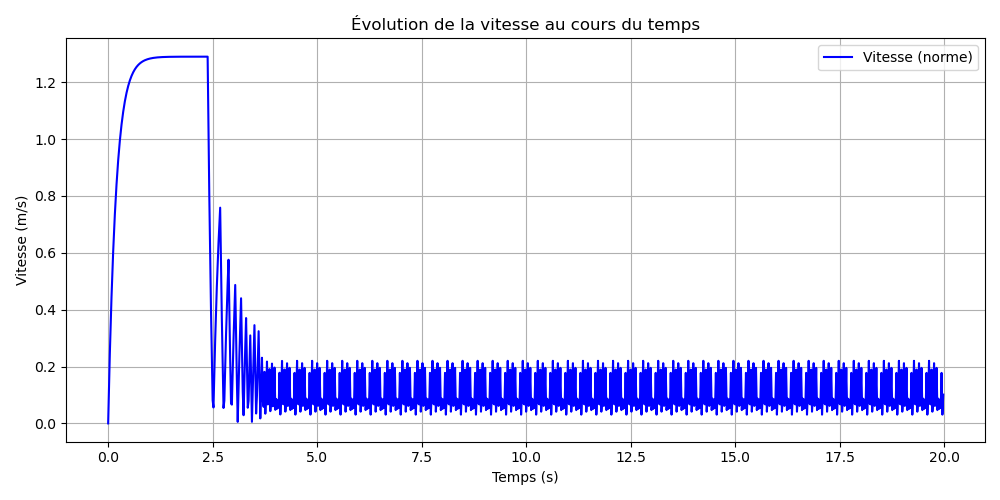
\includegraphics[width=\textwidth]{graph_vitesse.png} % moitié de la largeur du texte

Le résultat est bien cohérent on voit que la particule atteint à la manière d'une exponentielle inversé sa $v_{desiree}$ pour en suite l'atteindre totale. Dès que la position $(100,100)$ est atteinte sa vitesse décroit pour revenir vers la position. On voit qu'en suite la fonction devient périodique, la particule passe d'un bout à l'autre de la position (100,100) sans jamais l'atteindre.


\subsection*{Méthode de Runge-Kutta d'ordre 2}

Cette méthode plus couteuse temporellement s'avére être plus précise qu'euler.

L’équation générale est :
\[
\vec{v}_{n+1} = \vec{v}_n + k_2
\]
avec :
\[
k_1 = h \cdot \vec{F}(\vec{v}_n, \vec{r}_n)
\]
\[
k_2 = h \cdot \vec{F} \left( \vec{v}_n + \frac{1}{2}k_1, \vec{r}_n \right)
\]

\textbf{Dans le code :}
\begin{itemize}
    \item Le pas de temps est $h = 0{,}02$
    \item \texttt{k1} est calculé par :
    \[
    k_1 = h \cdot \texttt{resultante(tab\_personne, personne, indice, obstacles, portes)}
    \]
    \item Puis on modifie temporairement la vitesse :
    \[
    \vec{v} \mathrel{+}= \frac{1}{2} k_1
    \]
    \item Ensuite, on recalcule la force et :
    \[
    k_2 = h \cdot \texttt{resultante(...)}
    \]
    \item Enfin, on met à jour la vitesse avec :
    \[
    \vec{v}_{n+1} = \vec{v}_n + k_2
    \]
\end{itemize}
(voir code)
\begin{minted}[frame=single, bgcolor=white, linenos, breaklines=true]{python}
def runge_kutta_2(tab_personne, personne,indice,obstacles, portes, step=.02)
\end{minted}
\subsubsection{Resultats de rungge kutta 2 et 4}

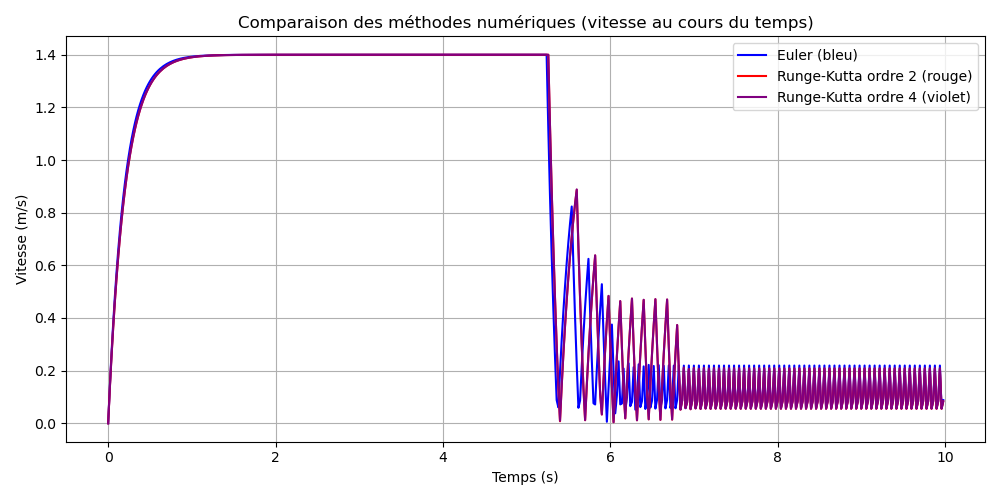
\includegraphics[width=\textwidth]{runge.png}

Au final, on observe un léger écart, dû à la plus grande précision de la méthode de Runge-Kutta. Mais cette écart sur la vitesse n'a pas un grans impact sur la position à en croire le graphique suivant:

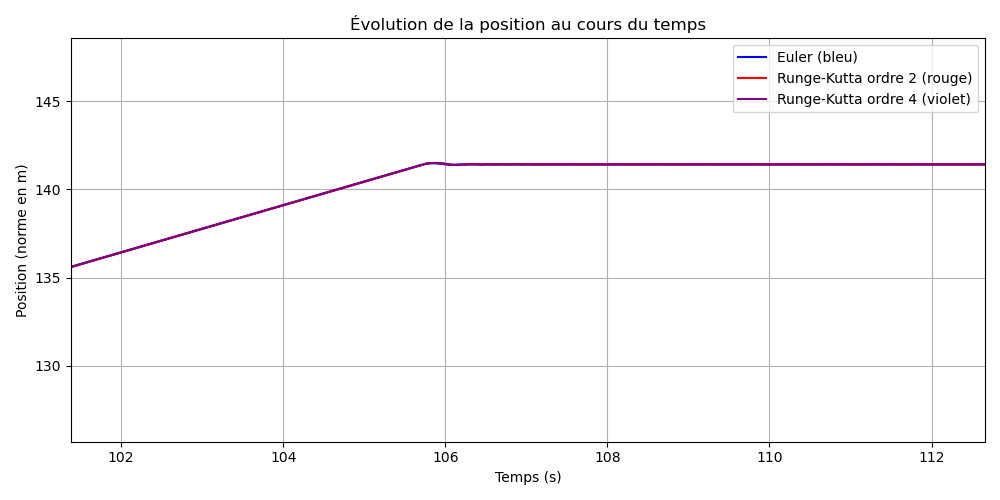
\includegraphics[width=\textwidth]{runge_pos.png}


\
\section{Explication du code}
\subsection{Structure et contextualisation}
\noindent Le code est divisé en trois modules distincts:
\begin{itemize}
	\item \textbf{main.py} s'occupe de dessiner la fênetre de gérer plusieurs actions il initialise le tableau de personne (tableau de particule)
	
	\item \textbf{physique.py} contient uniquement des fonction pour la gestion physique
	
	\item \textbf{affichage.py} contient les situations et centralise la gestion des dessin dans le canvas
\end{itemize}

\subsection{Modélisation physique}
Cette section présente les différentes fonctions du fichier \textbf{physique.py}, accompagnées de leur signature pour faciliter leur identification dans le code.
\subsubsection{Force motrice}

Pour caculer la force motrice on applique simplement \eqref{eq:force_motrice}

\begin{minted}[frame=single, bgcolor=white, linenos]{python}
def force_motrice(personne):
\end{minted}

La fonction \textbf{calcul\_i0} retourne le vecteur directionnel en soustrayant le point souhaité de la position actuelle de la personne, puis en normalisant le résultat comme suivant.
\\
\indent Soient $a$ la position de la particule et $ptSouhaite$ les coordonnées de la porte :
\begin{equation}
	\vec{e_\theta} = \vec{a} - \vec{ptSouhaite}
\end{equation}


\subsubsection{Force social(s)}


\begin{minted}[frame=single, bgcolor=white, linenos, breaklines=true]{python}
def force_intercation_social(tab_personne, personne, indice, b0=config["b0"], seuil_interaction=50)
\end{minted}

Pour caculer on applique \eqref{eq:force_sociale}
\\

Afin de limiter la complexité temporelle de la simulation, on ajoute deux conditions : une personne ne peut pas interagir avec elle-même (ce qui est logique d’un point de vue physique), et elle n’interagit qu’avec les autres personnes situées à moins de 50 unités de distance.  Ce seuil d’interaction (fixé à 50) est vérifiable physiquement une personne à une certaine distance d'un autre individu n'agissent pas deux à deux entre elle. A noté que cette valeur à été fixé expérimentalement.


Pour calculer $d_{ij}$ onprend la norme de la position de la personne avec la norme de la personne avec laquel elle intéragis on soustrait en suite les deux rayon qui correspond à $r_{ij}$. $\vec{n_{ij}}$ est le vecteur normal ( a - b ) qu'on norme pour avoir un vecteur unitaire. 


\subsubsection{Force répulsion mur}

\begin{minted}[frame=single, bgcolor=white, linenos, breaklines=true]{python}
def force_interaction_social_mur(personne, indice, portes, b0 = config["b0"]):
\end{minted}

La force de repulsion de mur est plus compliquée à calculer. Il faut la calculer pour chaque mur avec toujours un seuil d'intéraction (un mur agis sur nous que s'il nous touche). \textbf{$r_{ij}$} reste le même. Mais pour caculer \textbf{$d_{ij}$} cette fois ci on utilise pythagore.

\
La condition sert à ne pas agir si on a une porte.
\
La fonction \texttt{distance\_mur\_vect} utilise le théorème de Pythagore. Elle renvoie un tuple avec, premièrement, la distance entre le mur visé ($\mathbf{d_{ij}}$), ainsi que le vecteur normal ($\mathbf{n_{ij}}$). Pour mieux comprendre voici un exemple:

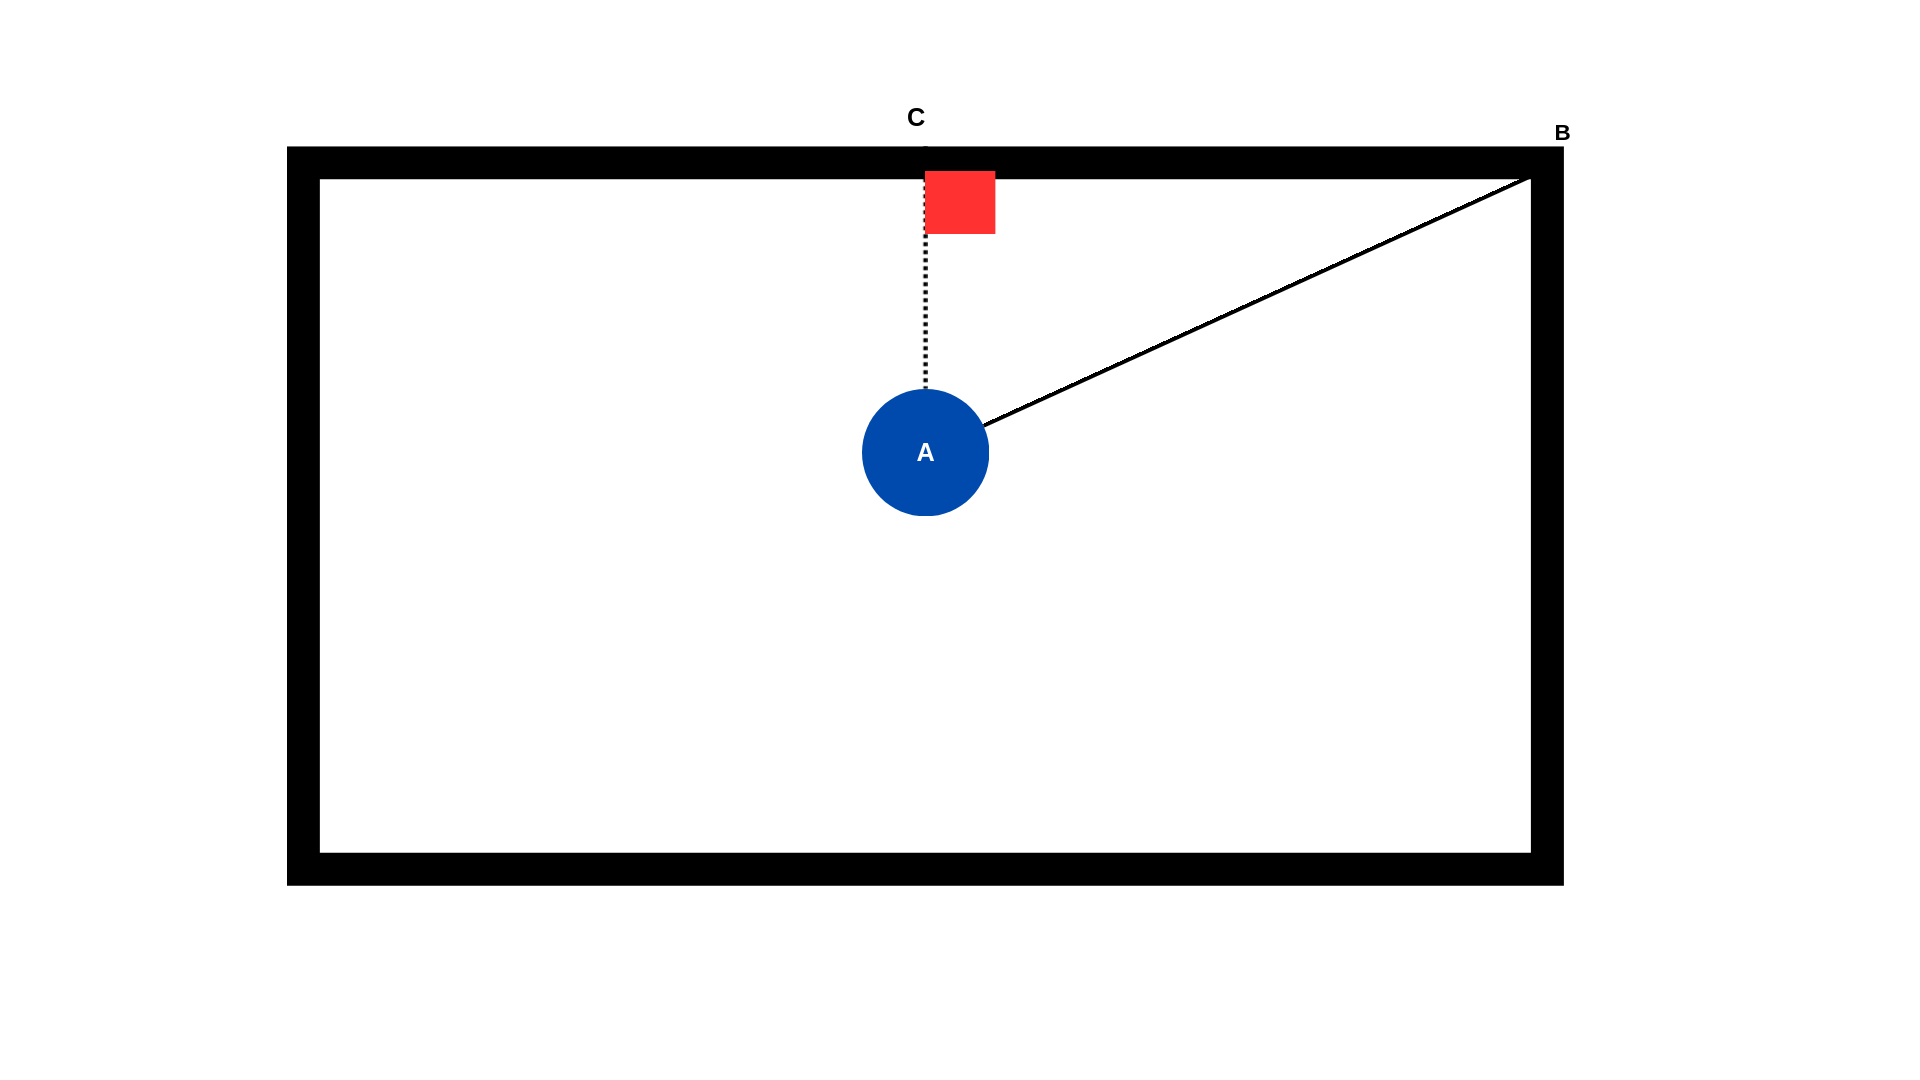
\includegraphics[width=\textwidth]{explication.png}

On a déjà la longueur \( AB \) et on cherche \( AC \), on obtient facilement l'angle \( \widehat{ABC} \) que l'on notera \( \alpha \). \\
On a alors : \( BC = \sin(\alpha) \cdot AB \)
\\
\\
Finalement d'après le théorème de pythagore $\sqrt{AB^2 - CB^2} = AC$, pour le vecteur normal on en déduit les coordonnés de c pour en suite normaliser $\vec{CA}$.
\\
\\
\indent Cette opération est répétée pour les autres murs de manière casi analogue. Une condition supplémentaire est ajoutée afin d’ignorer la zone correspondant à l’emplacement de la porte.

\subsubsection{Force interaction rectangle}

\begin{minted}[frame=single, bgcolor=white, linenos, breaklines=true]{python}
def force_intercation_rectangle(personne, rectangle, b0=config["b0"]):
\end{minted}

Pour cette méthode on a créé une fonction qui détermine le point le plus proche d'un rectangle. Selon la méthode suivante


\paragraph{Vecteurs de Projection :}

Soit un rectangle défini par ses coordonnées de coin inférieur gauche $(x, y)$, sa longueur $l$, et sa hauteur $h$. Nous définissons deux vecteurs :
\begin{itemize}
    \item $\vec{v}_{\text{longueur}} = (l, 0)$ : vecteur représentant la longueur du rectangle.
    \item $\vec{v}_{\text{hauteur}} = (0, h)$ : vecteur représentant la hauteur du rectangle.
\end{itemize}

\paragraph{Position Relative :}

La position de la personne par rapport au coin inférieur gauche du rectangle est:
\[
\vec{p}_{\text{relatif}} = (x_{\text{personne}} - x, y_{\text{personne}} - y)
\]

\paragraph{Projection sur les Bords du Rectangle :}

Pour trouver le point le plus proche sur le rectangle, on projette $\vec{p}_{\text{relatif}}$ sur les vecteurs $\vec{v}_{\text{longueur}}$ et $\vec{v}_{\text{hauteur}}$. On a donc:

\begin{align*}
k_1 &= \frac{\vec{p}_{\text{relatif}} \cdot \vec{v}_{\text{longueur}}}{\|\vec{v}_{\text{longueur}}\|^2} \\
k_2 &= \frac{\vec{p}_{\text{relatif}} \cdot \vec{v}_{\text{hauteur}}}{\|\vec{v}_{\text{hauteur}}\|^2}
\end{align*}

\paragraph{Ajustement des Projections :}

Les valeurs de $k_1$ et $k_2$ sont ajustées (pour s'assurer qu'elles se situent bien dans le rectangle) :
\begin{itemize}
    \item Si $k_1 < 0$, alors $k_1 = 0$.
    \item Si $k_1 > l$, alors $k_1 = l$.
    \item Si $k_2 < 0$, alors $k_2 = 0$.
    \item Si $k_2 > h$, alors $k_2 = h$.
\end{itemize}

\paragraph{Calcul du Point le Plus Proche :}

Le point le plus proche sur le rectangle est donc :
\[
\vec{p}_{\text{proche}} = (x, y) + k_1 \cdot \frac{\vec{v}_{\text{longueur}}}{\|\vec{v}_{\text{longueur}}\|} + k_2 \cdot \frac{\vec{v}_{\text{hauteur}}}{\|\vec{v}_{\text{hauteur}}\|}
\]

Pour finir on applique \eqref{eq:force_sociale} ici $r_{ij}$ = $r_i$ - 0 car pas de rayon.

\subsection{Resolution}

\textbf{Situation 1}

Bilan des forces :
Trois types de forces principales agissent sur l’individu :
\begin{itemize}
\item \textbf{Les forces motrices}, modélisées par l’équation \eqref{eq:force_motrice} ;
\item \textbf{Les forces d’interaction entre personnes}, données par \eqref{eq:force_sociale} ;
\item \textbf{Les forces d’interaction avec les murs}, également représentées par \eqref{eq:force_sociale}.
\end{itemize}

On peut également intégrer les interactions avec d’autres obstacles. Dans le cas où aucun obstacle n’est présent, le vecteur de force associé sera simplement nul : $\vec{0}$.

\vspace{1em}

Ainsi, on peut généraliser le système via une fonction basée sur la méthode d’Euler (et de Runge-Kutta), capable de traiter l’ensemble des cas évoqués.

\vspace{1em}

C'est ce que font les fonctions de résolutions suivantes.

\begin{minted}[frame=single, bgcolor=white, linenos, breaklines=true]{python}
def runge_kutta_2(tab_personne, personne,indice,obstacles, portes, step=.02):
def runge_kutta_4(tab_personne, personne,indice,obstacles, portes, step=.02):
def euler(tab_personne, personne,indice,obstacles, portes, step=.02):
\end{minted}


\section{Analyse}
Le temps de notre expérience est en unités de temps il ne dépend pas de la puissance de l'ordinateur pour un résultat plus fiable c'est seulement un incrément à chaque étape de la modélisation. Les différences observées sont dû à la vitesse qui varie de $1.34 \pm 0.25 m.s^{-1}$
\subsection{Situation 1}

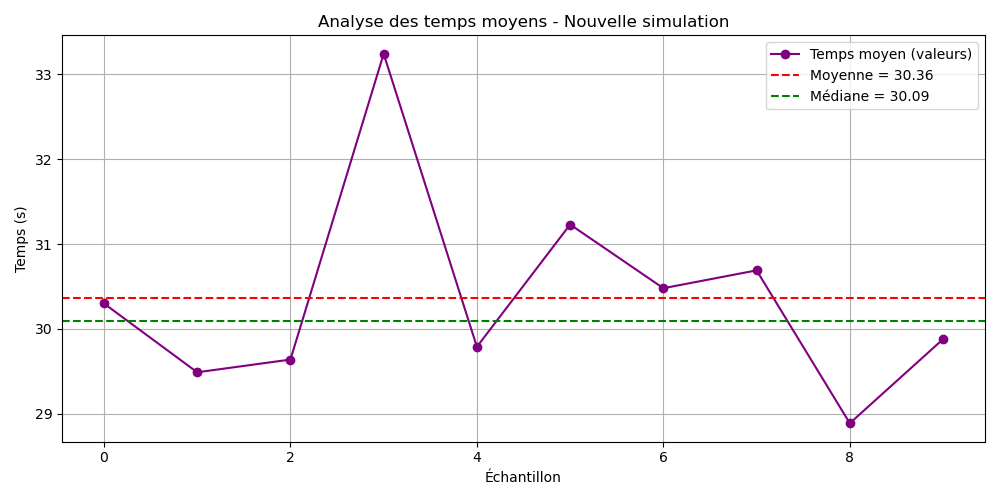
\includegraphics[width=\textwidth]{resultat.png} % moitié de la largeur du texte
Sur un échantillonage de 10 valeurs
\\
\\
Pour cette simulation on obtient un temps moyen de \textbf{30.36 unités de temps}.
\subsection{Situation 2}


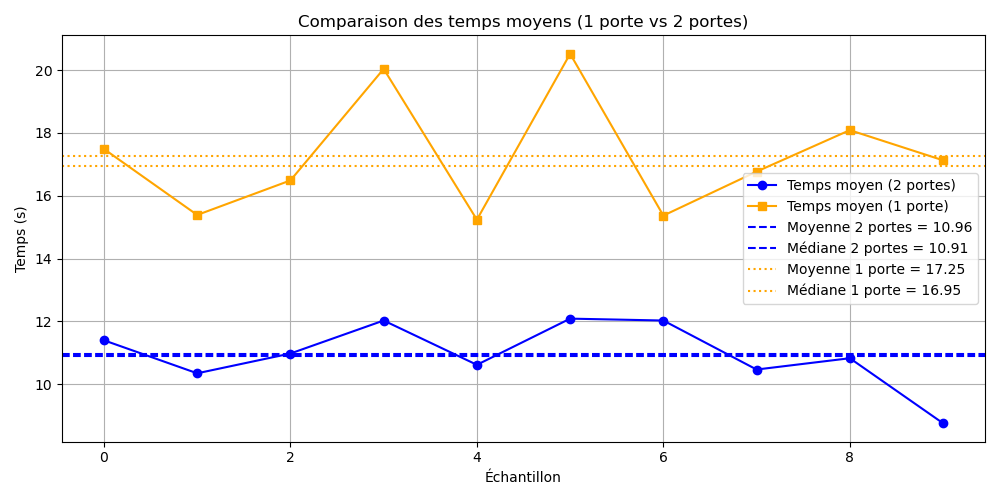
\includegraphics[width=\textwidth]{resultat_2.png} % moitié de la largeur du texte

On obtien une moyenne de temps sur 10 échentillons pour la classe avec 2 portes de 10.96 unité de temps tandis qu'avec 1 porte la moyenne est de 17.25 unité de temps. Pour ramener sur une echelle plus parlante que des unités de temps dans le cas ou il y a seulement une porte le temps sera augmenté d'environ \textbf{61\%}. 
\paragraph{Conclusion}  Une telle augmentation peut avoir des conséquences critiques en situation d'urgence, car chaque seconde supplémentaire est un risque, en particulier en cas de panique ou de mouvements de foule. \\ \indent A noter que notre model aurait pu être plus proche de la réalité en ajoutant le principe de décision individuel pour avoir des chemins différents.
\newpage



\section{Réferences}


\vspace{1em}

\begin{itemize}
	\item \href{https://journals.aps.org/pre/abstract/10.1103/PhysRevE.51.4282}{Social force model for pedestrian dynamics (Dirk Helbing et Péter Molnár)}
	\item \href{https://github.com/antoninnad/etude_des_foules}{Lien vers le dépo git}
\end{itemize}

\end{document}

\end{document}


pdflatex -shell-escape index.tex



